
\section{Machine learning module}
\subsection{Dataset source}
The dataset used is gotten from \href{https://www.kaggle.com/datasets/fedesoriano/heart-failure-prediction}{kaggle} and was made by putting together different datasets that were already out there but had never been put together before. In this dataset, 5 heart datasets are put together based on 11 common features. This makes it the largest dataset for heart disease research that has been made available so far. The five datasets that were used to put it together are:
\begin{enumerate}[label=(\alph*)]
	\item Cleveland: 303 observations
	\item Hungarian: 294 observations
	\item Switzerland: 123 observations
	\item Long Beach VA: 200 observations
	\item Stalog (Heart) Data Set: 270 observations
\end{enumerate}

\comment{The classification process was carried out with the use of k-nn, naive bayes, decision tree, and logistic regression algorithms.}

\subsection{Exploratory data analysis}

\subsubsection{Correlation matrix}
A correlation matrix is nothing more than a table that displays the correlation coefficients for various variables. The matrix illustrates the relationship between all possible pairings of values in a table. It is a strong tool for summarizing a large dataset as well as identifying and visualizing trends in the data. The code to produce the matrix can be seen in \ref{lst:corr}.


\begin{figure}[htb]
	\centering
	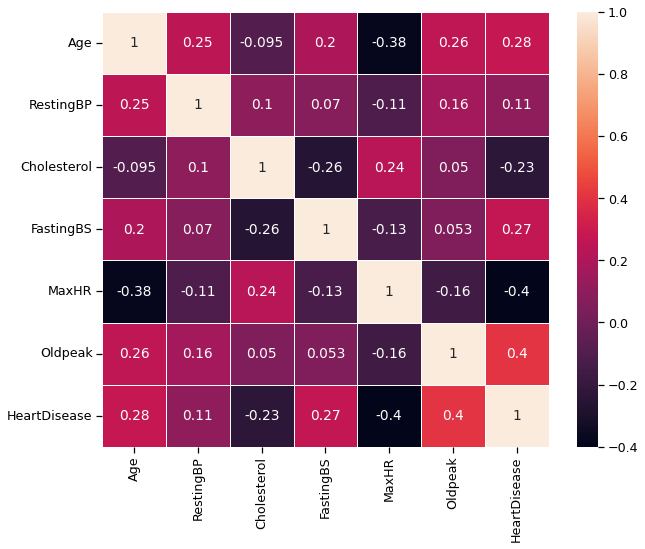
\includegraphics[scale=0.65]{correlation-chart.png}
	\caption{Correlation matrix}
	\label{fig:correlation-chart}
\end{figure}
From the correlation chart \figurename~\ref{fig:correlation-chart} we can see that:
\begin{enumerate}[label=(\roman*)]
	\item{Oldpeak is highly positively correlated to the target variable.}
	\item{MaxHR is highly negatively correlated toe the target variable.}
	\item{RestingBP has the lowest correlation compared to other attributes}
\end{enumerate}
\subsubsection{Plotting numerical values}
In Listing~\ref{lst:plot-numerical} I plotted age and fasting blood sugar count with the target column.

\comment{
\begin{figure}[htb]
	\centering
	\begin{floatrow}
		\ffigbox[\FBwidth]{\caption{Ages chart}\label{}}{
			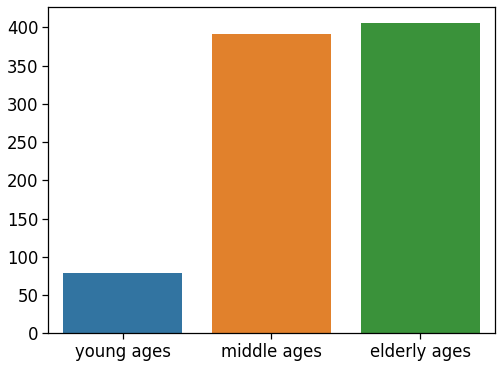
\includegraphics[scale=0.4]{ages-chart.png}}
		\ffigbox[\FBwidth]{\caption{FastingBS chart}\label{}}{
			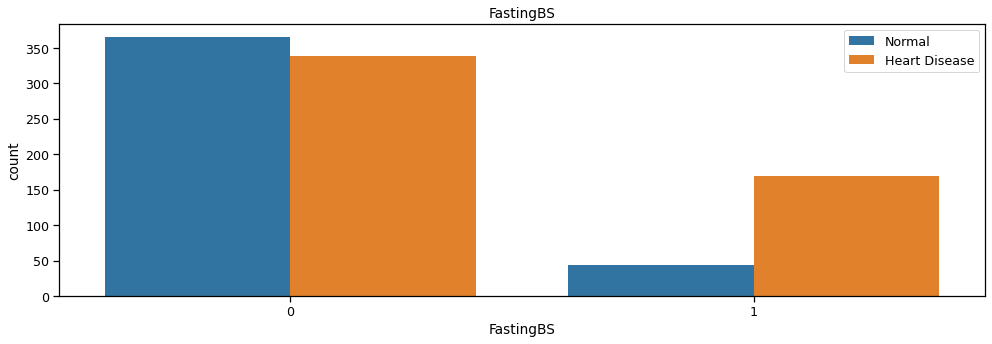
\includegraphics[width=3in, height=3in]{fasting-bs-chart.png}}
	\end{floatrow}
\end{figure}
}

\begin{figure}[htb]
	\centering
	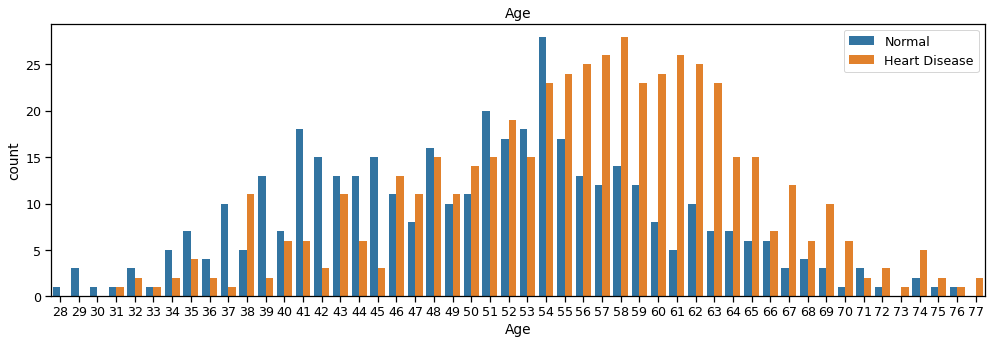
\includegraphics[scale=0.45]{age-count-chart.png}
	\caption{Age}
	\label{fig:age-count-chart}
\end{figure}
We can see that in \figurename~\ref{fig:age-count-chart} the occurrence of heart disease in the older ages from 55 to 77 is higher.

\begin{figure}[htb]
	\centering
	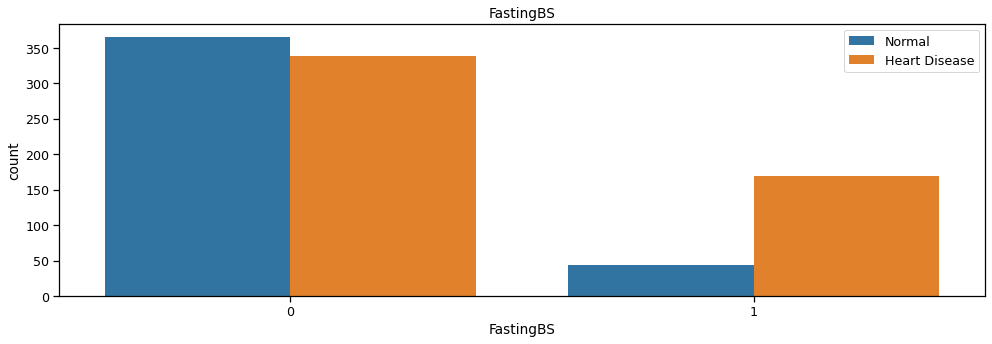
\includegraphics[scale=0.45,]{fasting-bs-chart.png}
	\caption{Fasting blood sugar}
	\label{fig:fasting-bs-chart}
\end{figure}

From the figure in ~\ref{fig:fasting-bs-chart} we can infer that higher fasting blood sugar is more likely to have heart disease.
\subsubsection{Plotting categorical values}
In listing \ref{lst:plot-categorical}, the categorical attributes of the dataset are plotted.

\begin{figure}[htb]
	\centering
	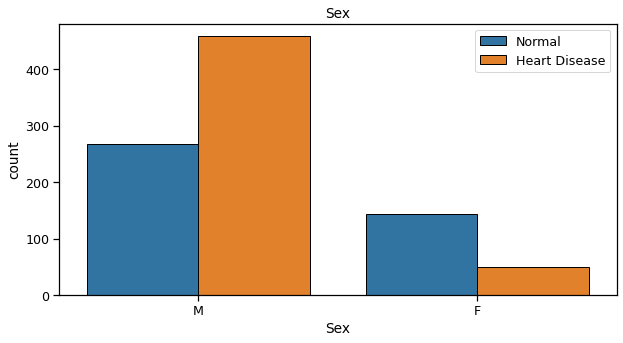
\includegraphics[scale=0.45]{sex-chart.png}
	\caption{Sex}
	\label{fig:sex-chart}
\end{figure}

From \figurename~\ref{fig:sex-chart} we can see that there is more occurrence of heart disease in males than females.

\begin{figure}[htb]
	\centering
	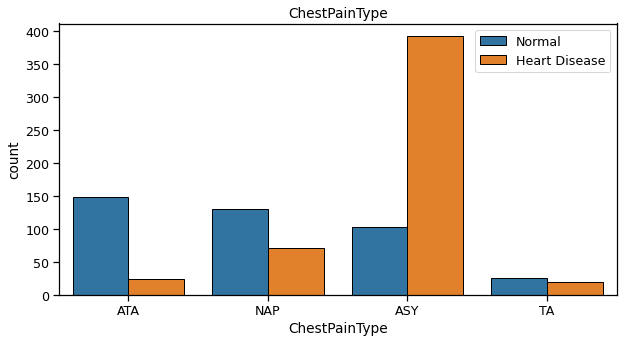
\includegraphics[scale=0.45]{chestpaintype-chart.png}
	\caption{Chest pain type}
	\label{fig:chestpaintype-chart}
\end{figure}
We can see from \figurename~\ref{fig:chestpaintype-chart} that the Asymptomatic chest pain type is highly correlated with heart disease.

\begin{figure}[htb]
	\centering
	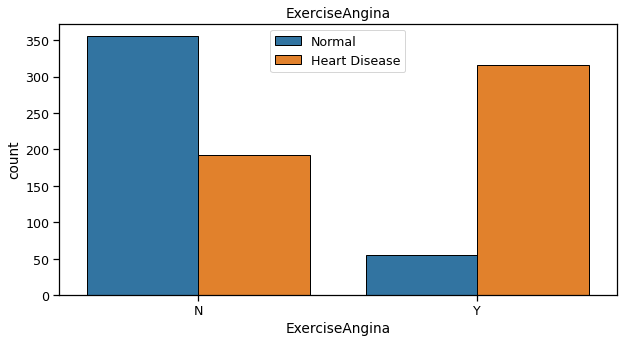
\includegraphics[scale=0.45]{exercise-angina-chart.png}
	\caption{Exercise angina}
	\label{fig:exercise-angina-chart}
\end{figure}

\begin{figure}[htb]
	\centering
	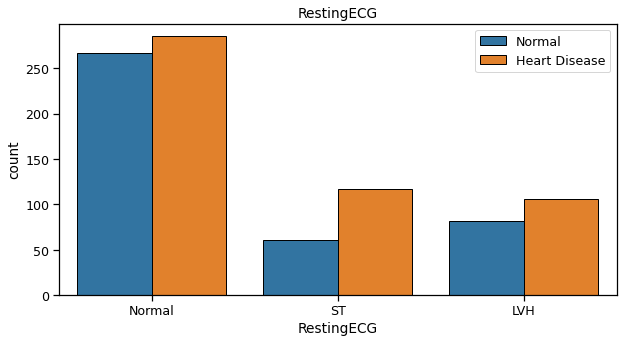
\includegraphics[scale=0.45]{restingecg-chart.png}
	\caption{Resting electrocardiogram results}
	\label{fig:restingect-chart}
\end{figure}

\subsection{Data preprocessing}
The preprocessing steps in the following subsections were applied on the dataset.
\subsubsection{Imputation}
Before imputation, we have to check for missing values in the dataset using \lstinline[language=Python,columns=fixed]|df.info()|. The output can be seen in listing \ref{lst:dataset-info-output}. We can see from the output that there are no null values in the dataset.


\subsubsection{Feature scaling}
Feature scaling was done using the MinMaxScaler class in the sklearn library on the dataframe used to train non-tree based algorithms. The source can be seen in listing~\ref{lst:min-max-scaler}.


\subsubsection{Handling of categorical values}
Label encoding is used in this study for Decision tree model while One-Hot encoder is used for the non-tree based algorithms shown in listing~\ref{lst:label-encoding} and listing~\ref{lst:one-hot-encoding} respectively.




\subsection{Training and Performance analysis}
The dataset was split using StratifiedKFold over 5 folds for cross validation and the accuracy of every fold was calculated using area under the ROC curve (AUC) to get precision, recall and f1-score.


\subsubsection{Logistic Regression}
Logistic regression had a peak accuracy of 88\% after cross-validation

\subsubsection{Naive Bayes}
Naive Bayes had a peak accuracy of 88.3\% after cross-validation

\subsubsection{KNN}
K-nearest neighbours had a peak accuracy of 91.6\% after cross-validation

\subsubsection{Decision Tree}
Decision Tree had a peak accuracy of 77.2\% after cross-validation

\section{Web Server module}
The web server contains the views and the inference engine. The views module is responsible for responding to http request from a client. The home page displays a form \figurename~\ref{fig:site-2} for the user to enter the medical data. When the data form is sent, the server processes the data and returns the results and inference in the result page, \figurename~\ref{fig:site-3}. The entrypoint to the main application can be found in listing~\ref{lst:web-server-entrypoint}


\begin{figure}[htb]
	\centering
	\makebox[0cm]{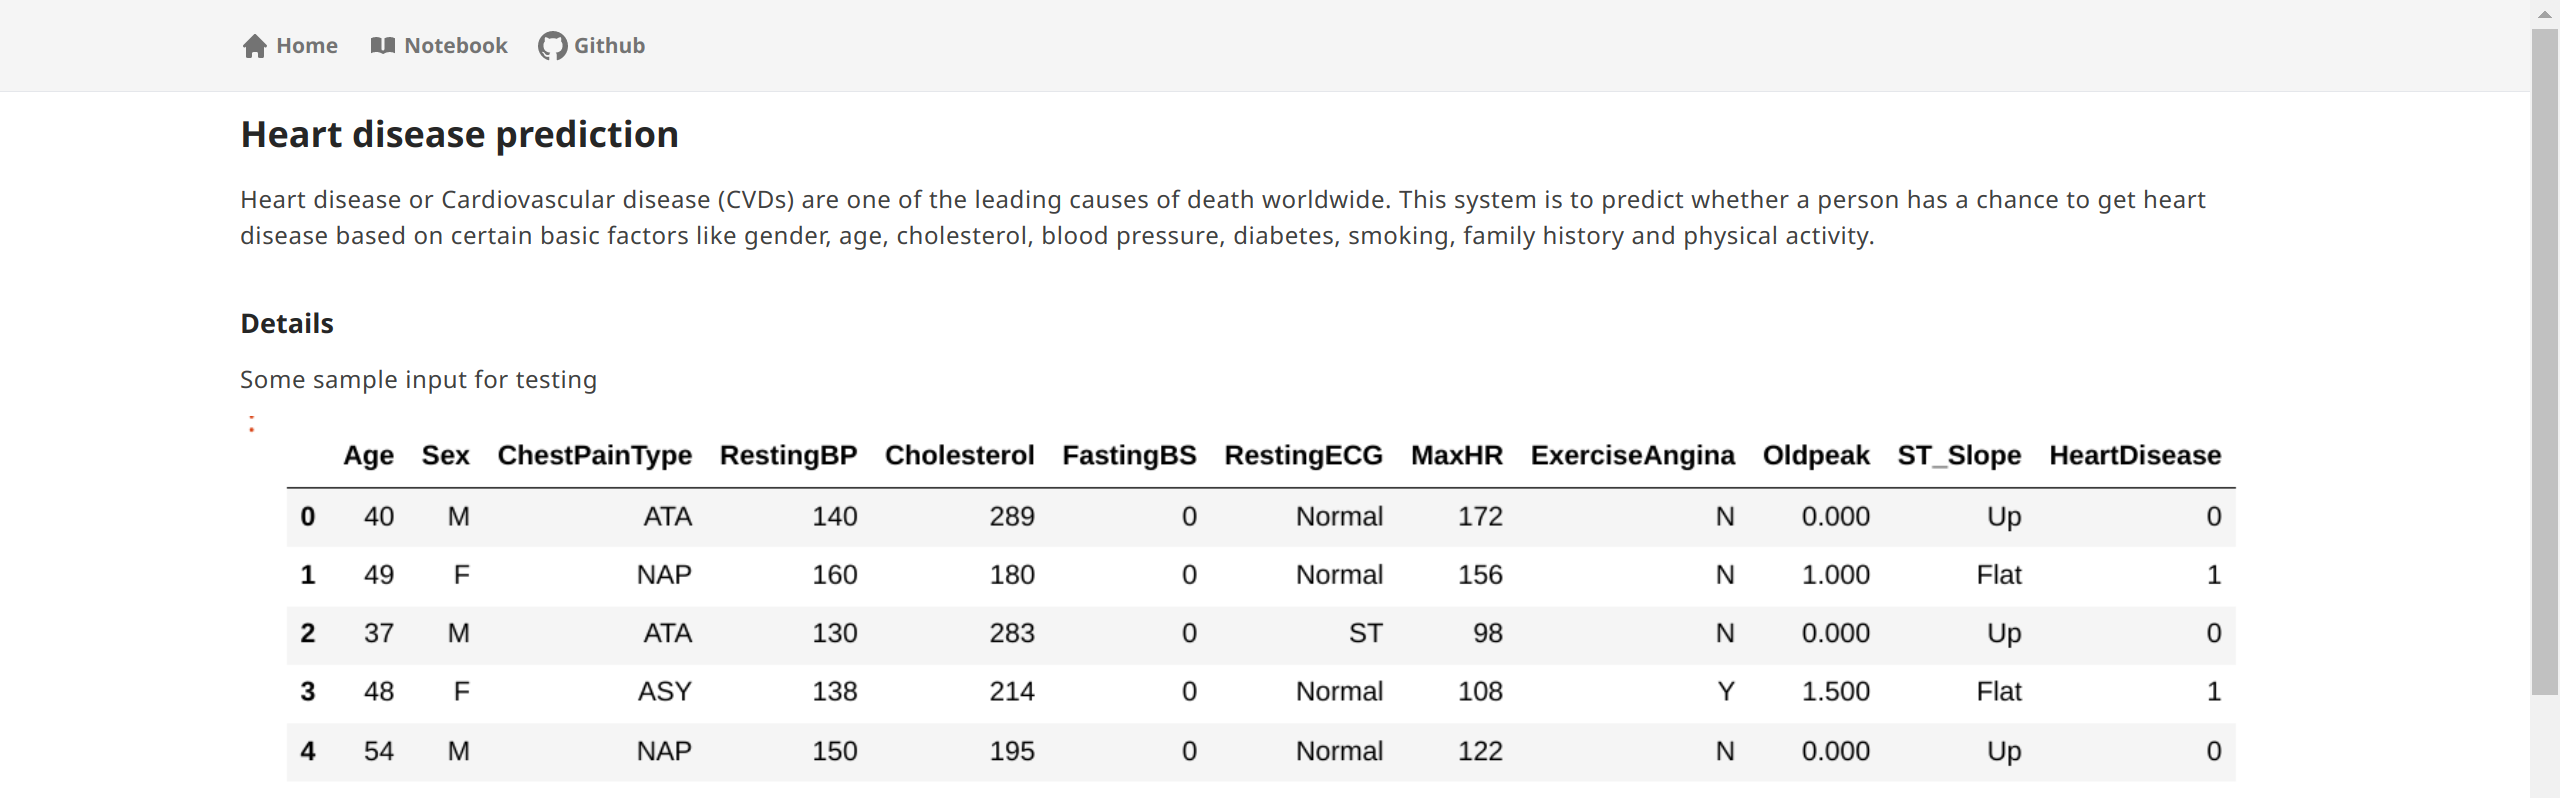
\includegraphics[scale=0.5]{site-1.png}}
	\caption{Webpage top}
	\label{fig:site-1}
\end{figure}

\begin{figure}[htb]
	\centering
	\makebox[0cm]{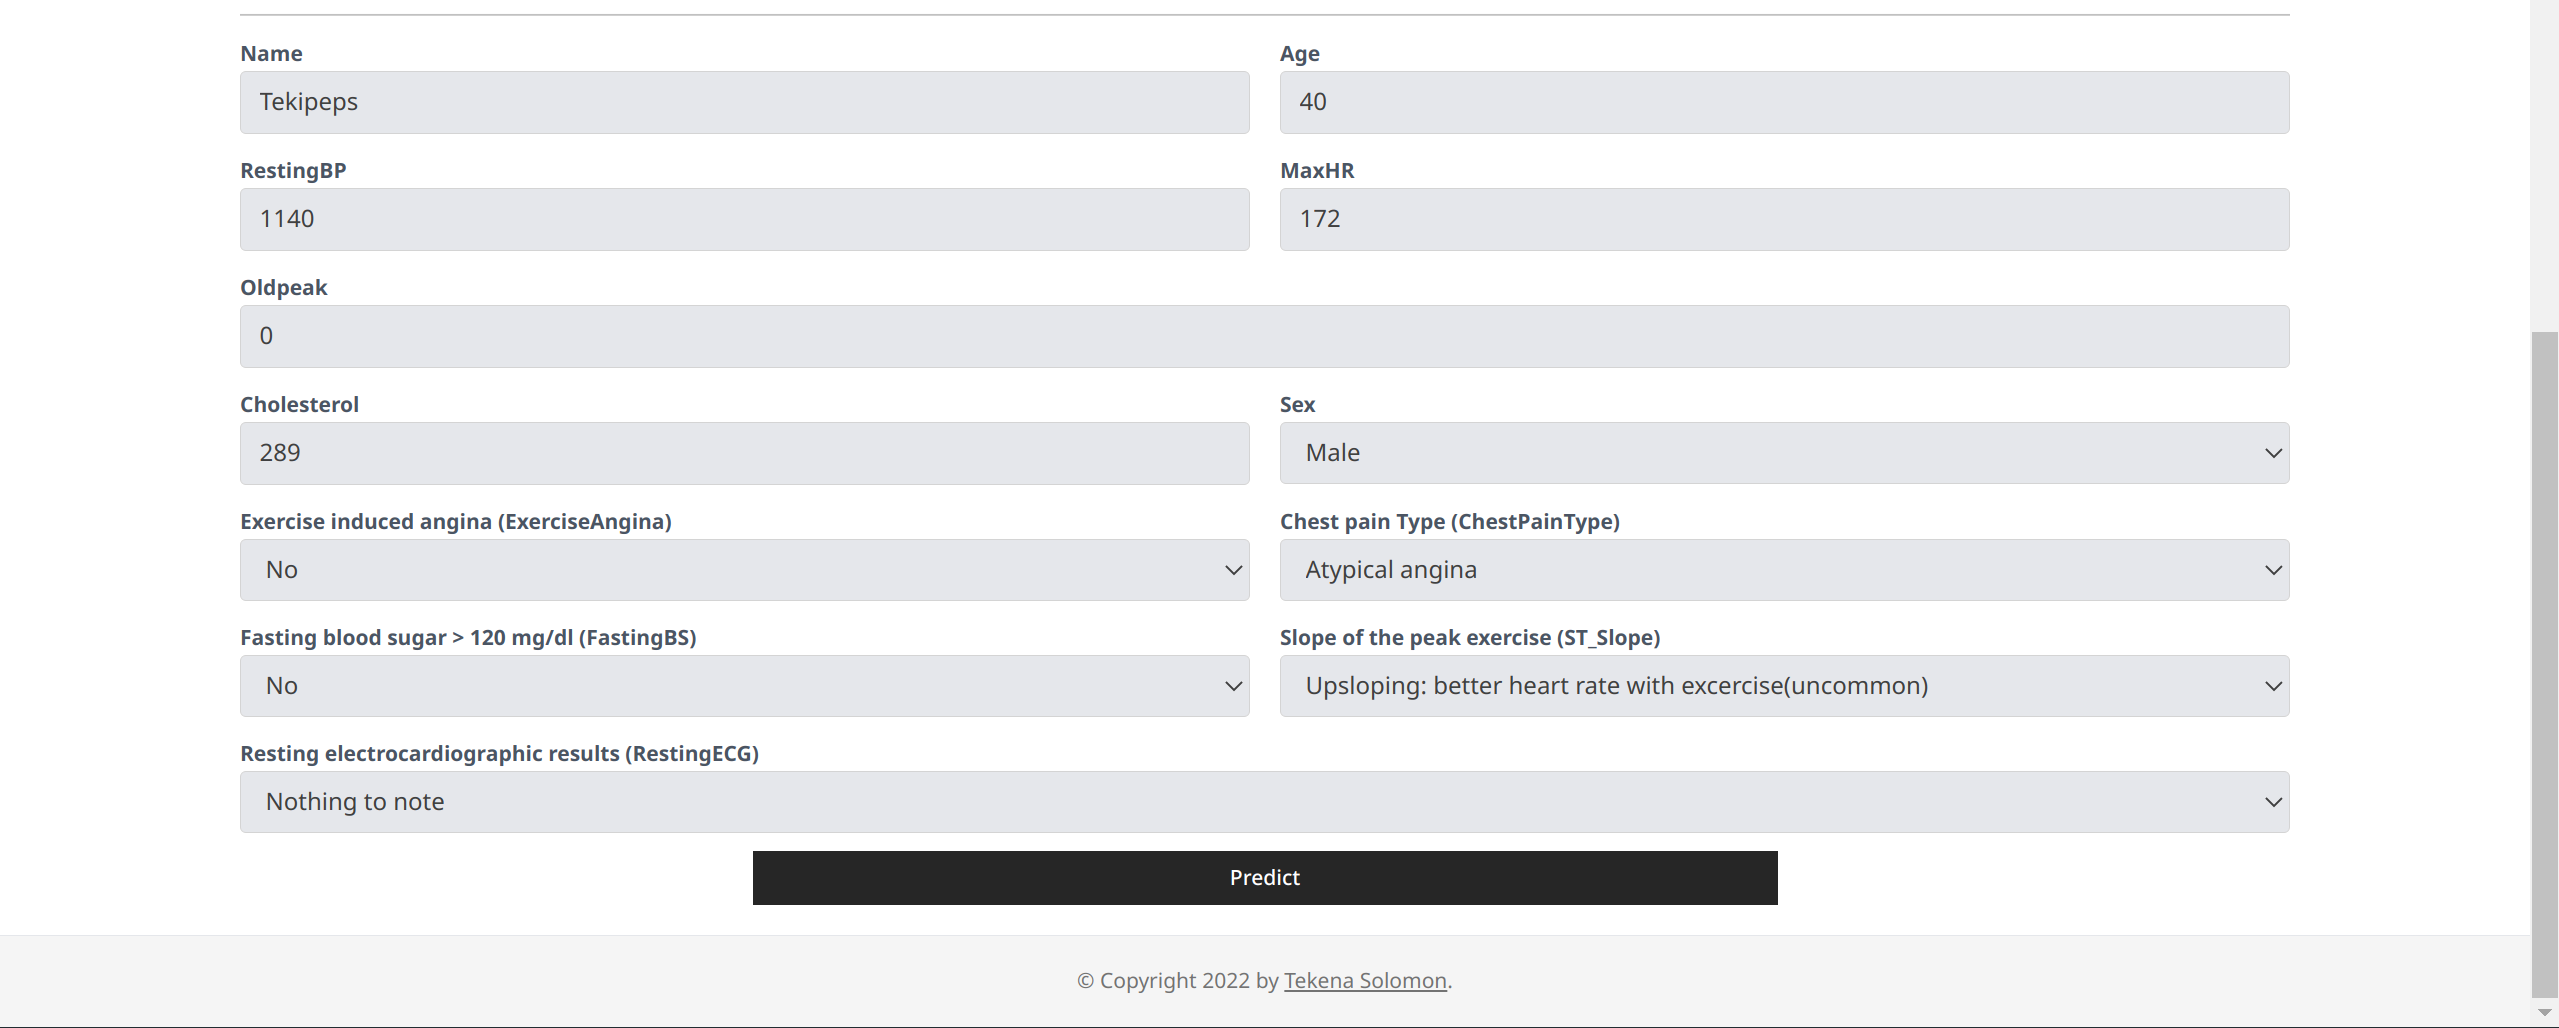
\includegraphics[scale=0.5]{site-2.png}}
	\caption{Webpage form}
	\label{fig:site-2}
\end{figure}
\begin{figure}[htb]
	\centering
	\makebox[0cm]{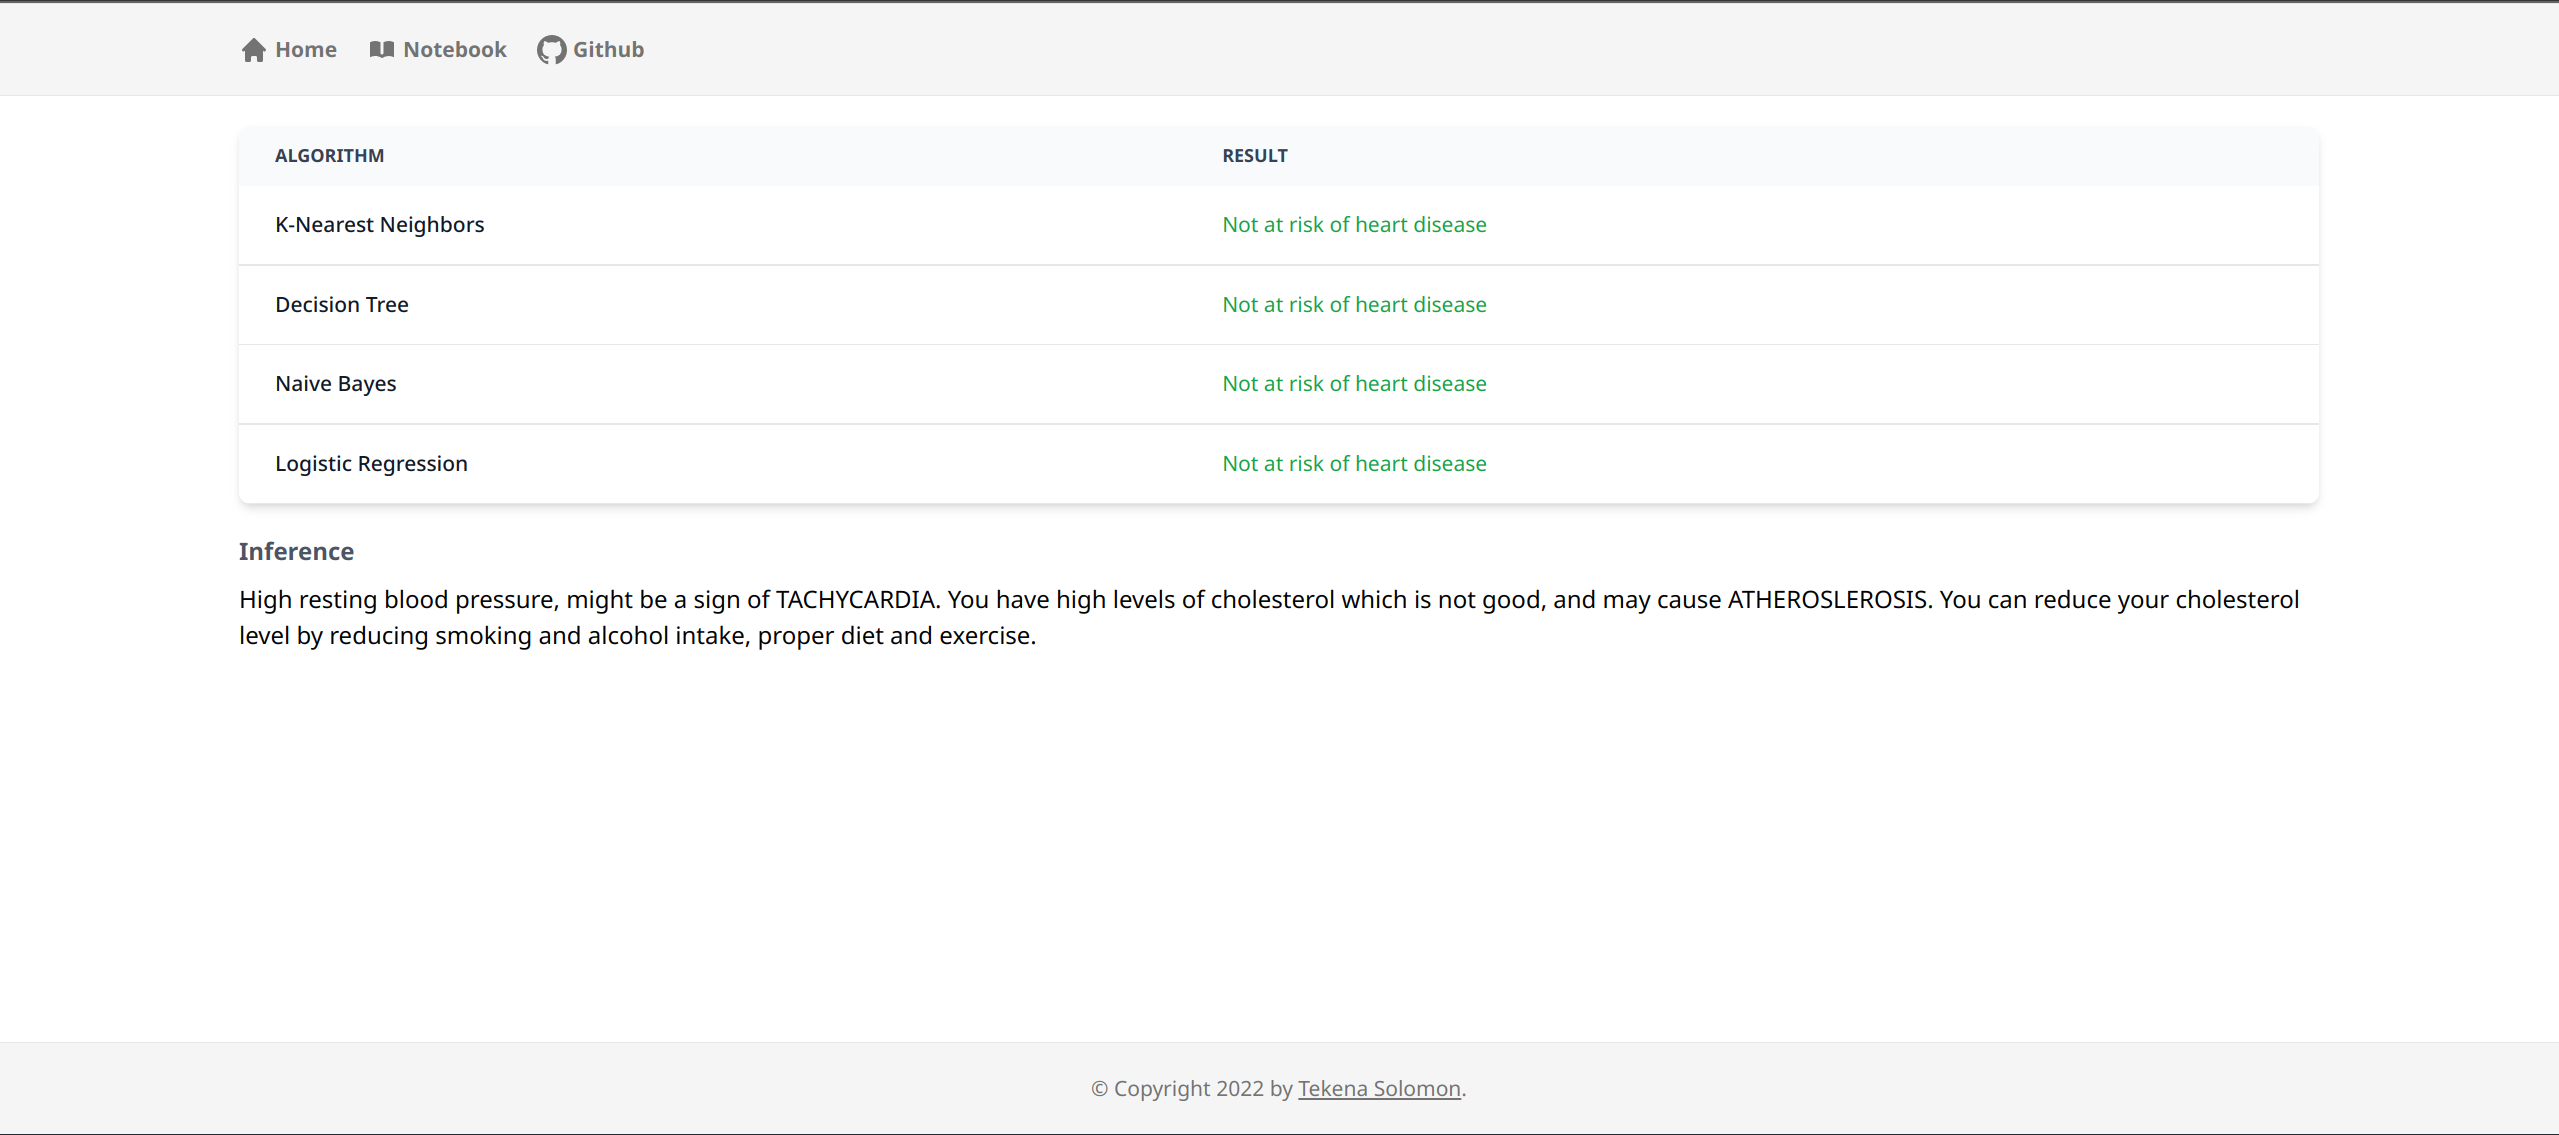
\includegraphics[scale=0.4]{site-3.png}}
	\caption{Results page}
	\label{fig:site-3}
\end{figure}



\section{Inference engine module}
The inference engine module is responsible for producing inference on the medical data. It consists of the knowledge base and the parser.

\subsection{Knowledge base}
The knowledge base is encoded in yaml format. It contains the attributes and conditions (rules) on those attributes that produce an inference. The knowledge base is shown in \figurename~\ref{fig:kb}

\begin{figure}[htb]
	\centering
	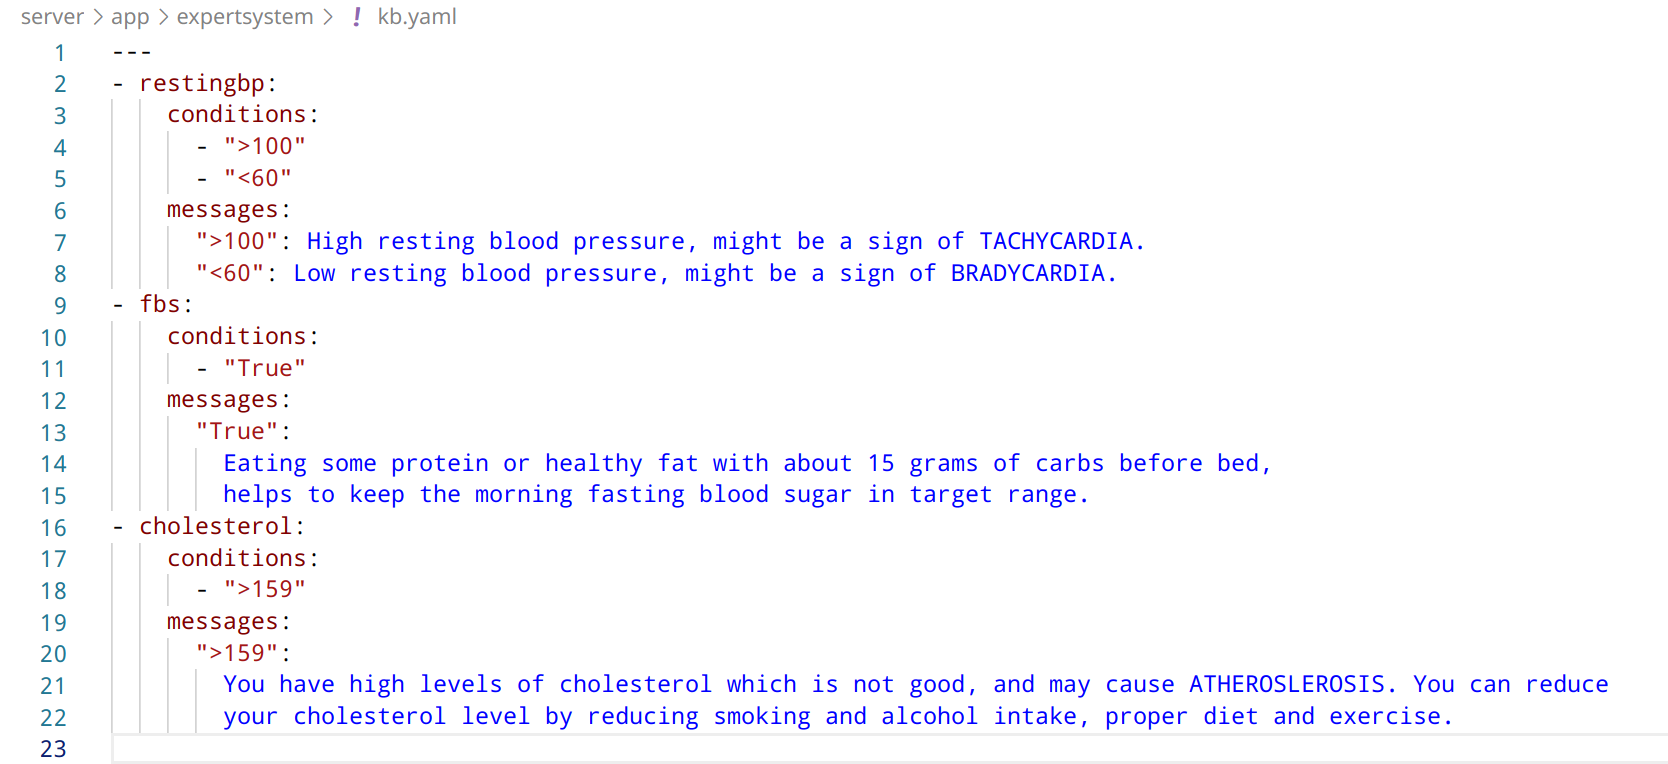
\includegraphics[scale=0.67]{kb.png}
	\caption{Knowledge base}
	\label{fig:kb}
\end{figure}

\subsection{Parser}
The parser parses the knowledge base and provides output based on the medical data. The parser takes the medical data as a lookup table to be able to call the values while parsing. The parser implementation is shown in listing~\ref{lst:kb-parser}

